\section{Optimal Controller}
\label{sec:idealcontroller}

% Theoretical
Consider a theoretically optimal controller for positioning the arm.
It would drive the motor with as much power as possible to accelerate the arm when a new position is desired.
At a critical point, it would reverse the polarity of the motors power-supply and apply as much power as possible to decelerate it.
This deceleration would continue and end only once the arms velocity reaches zero.
The critical point should be such that when the arms velocity reaches zero and the power supply switches off (no further acceleration), the arm is positioned exactly where it should be. 
As described, the motor controllers output would always be saturated (or zero), it would switch polarity only once each time a new position is requested, and there would be no overshoot of the arms position. 
Practically, implementing this behavior exactly is nearly impossible as it allows for no error and variability.

Based on the above mentioned criteria for optimality, the controller created for this project comes amazingly close realizing perfect performance.
The output of the controller after voltage conditioning, captured during an experiment and shown saturated at the limits where the H-bridge always drives the motor one direction, can be seen in Figure \ref{fig:idealcontroller}.
Over the entire course of the experiment, with the exception of returning to zero, only the areas indicated by the A and B labels show non-optimal controller behavior.
These pick-up and drop-off locations, are very narrow compared to the rest of the signal, which implies that the system control is close to optimal.
% More?

\begin{figure}[htp]
    \centering
    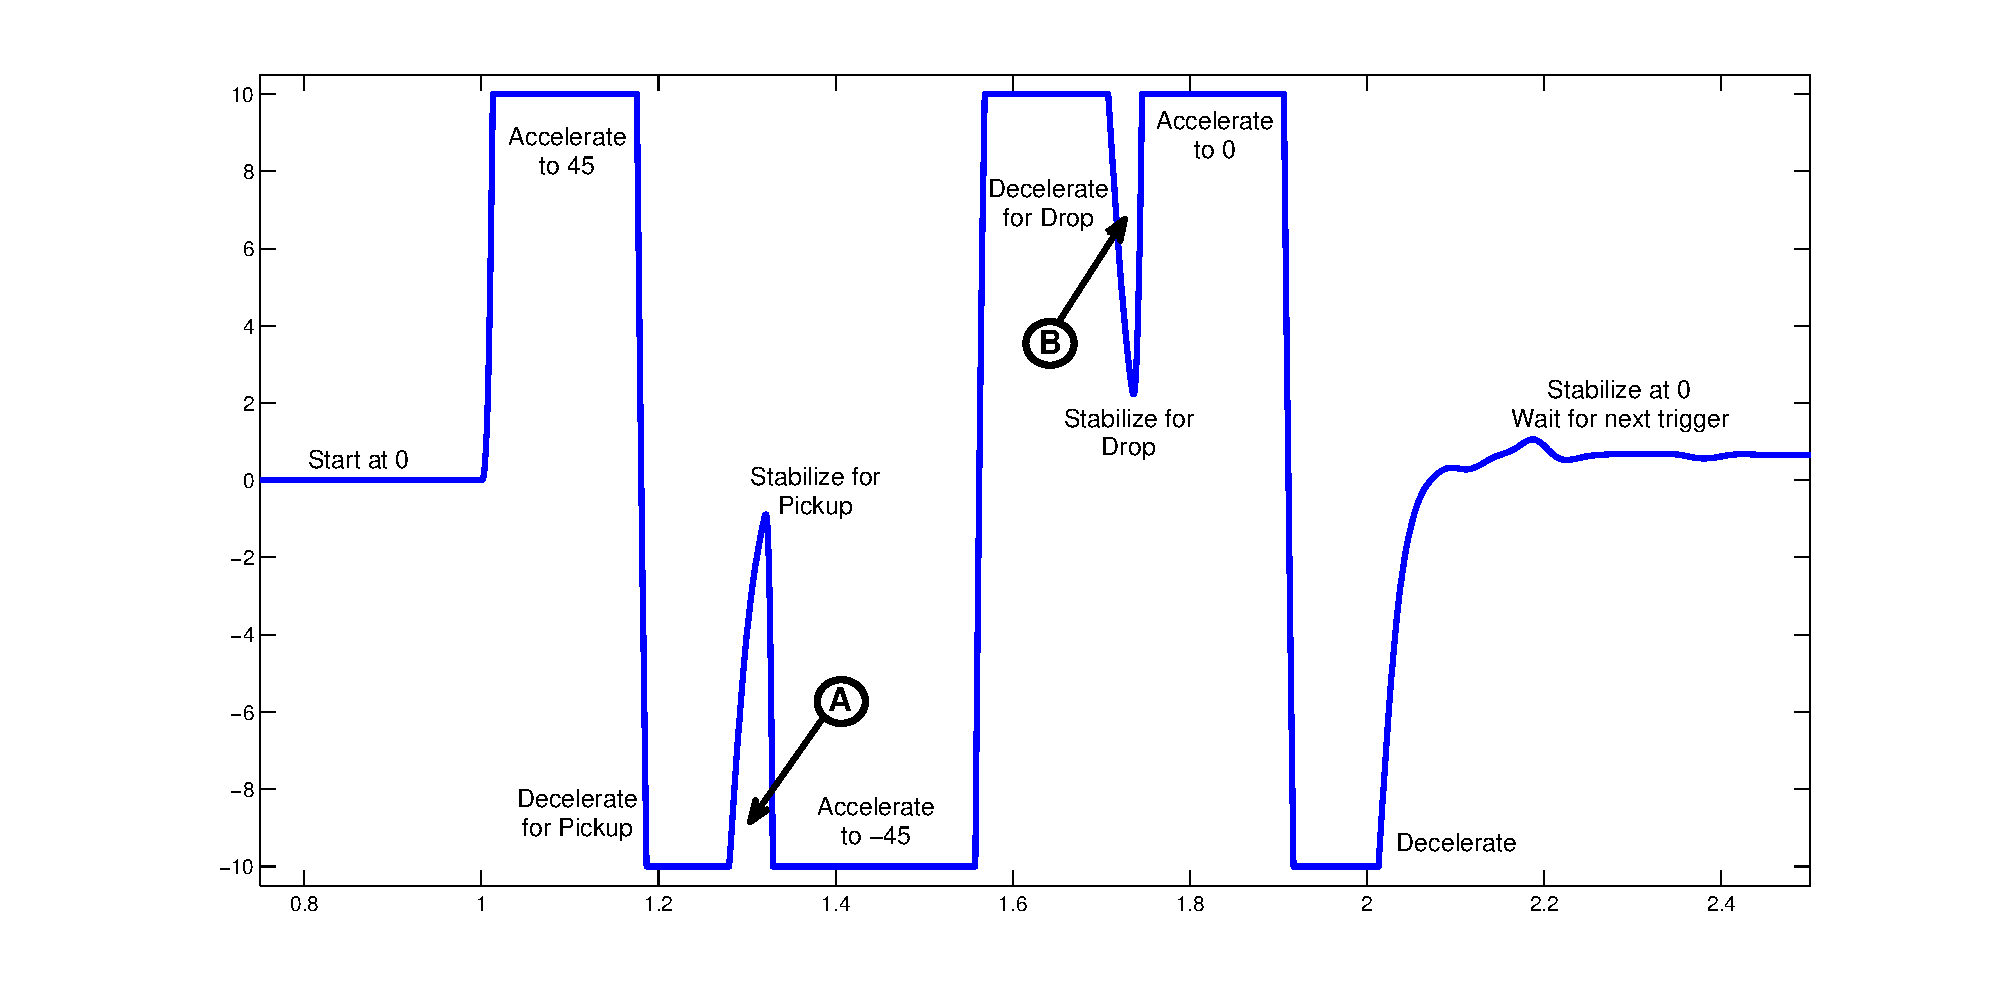
\includegraphics[width=.95\textwidth]{images/IdealControllerVoltage.pdf}
    \caption{Controller Output (Voltage)}
    \label{fig:idealcontroller}
\end{figure}


% PID 
Two approaches may be used to achieve the optimal controller within the limits of a PID.
First, a simple PID controller can be used with very large gains such that the controller output saturates the PWM input.
The disadvantage of this technique is that the standard analytical techniques used to design a PID are no longer valid. 
Additionally, very large gains increase the natural frequency of the system, increasing the risk of undesirable interaction with the relatively low frequency software PWM (see section \ref{sec:swpwm}).
The second approach, used in this project is to switch controllers based on the error signal. 
The general logic is as follows.

\begin{enumerate}

\item \textbf{P} - 
When the error signal is large, or the truss is positioned far from where it should be, use a purely proportional controller.
This decreases response time and saturates the motor controller immediately. 

\item \textbf{PD} - 
When the error signal reaches a critical threshold, switch to a slightly over-damped PD controller to slow the system down and perform final positioning.
This threshold should be less than the optimal threshold discussed above such that error feedback may be used to correct for inaccuracy and system variation.

\item \textbf{PID} - 
Finally, when the error signal is relatively small, add integral gain to correct for any steady state error.

\end{enumerate}


%The challenge of proportional control  is reaching a desired output quickly, while avoiding overshoot and minimizing ripple once it gets there. 
%Responding quickly suggests the need for a high proportional gain, while on the other hand, minimizing overshoot and oscillation suggests a small proportional gain. 
%To overcome this issue, the system begins by accelerating with a simple P gain to achieve maximum motor speed (saturation 10V) and therefore shortest time to reach the desired pick-up position at 45 deg. 
%As it decelerates for pick-up in region A, a PD controller is implemented to decrease maximum overshoot, rise time, and settling time. 
%Finally, an integral gain is added when the signal is small to reduce the steady-state error. The figure below shows the output that was achieved. 


%See figure \ref{fig:idealcontroller}.

